\documentclass[10pt,a4paper]{article}
\usepackage[utf8]{inputenc}
\usepackage{amsmath}
\usepackage{wallpaper}
\usepackage{amsfonts}
\usepackage{amssymb}
\usepackage{graphicx}
%\usepackage[style=alphabetic]{biblatex}
\usepackage{listings}
\lstset{language=matlab}

\begin{document}
\begin{titlepage}
\begin{center}
\vspace*{1cm}
\Huge
\textbf{Percolazione}
\vspace{0.5cm}
\LARGE
\\
Implementazione algoritmo HK per ricerca cluster percolante e benchmark con algoritmo "label" 
        
\vspace{1.5cm}
\textbf{Ayoub Ouarrak}
\vfill
        
\vspace{0.8cm}
\begin{center}
\includegraphics[width=4.0cm]{Unipr.png} 
\end{center}
\Large
Dipartimento di Matematica e Informatica\\
Universtità degli studi di Parma\\
2013/2014        
\end{center}
\end{titlepage}
\newpage
\tableofcontents

\newpage
\section{Definizione}
Chiamiamo reticolo una struttura formata da \emph{siti}, i quali possono essere vuoti oppure pieni con probabilità \emph{p}, definiamo \emph{cluster} un gruppo di siti pieni, in cui ogni sito è adiacente ad un'altro sito ai lati, in alto oppure in basso.\\
\begin{center}
\includegraphics[width=6.0cm]{cluster.png}
\end{center}
Un cluster viene chiamato percolante se attraversa l'intero reticolo passando dalla parete sinistra verso la perete destra
\section{Individuazione cluster percolante}
\subsection{Generazione matrice}
Per generare il reticolo, utilizzeremo la funzione rand di matlab, per ottenere inizialmente una matrice formata da valori compresi tra 0 e 1, successivamente verrà creata una matrice di zeri che verra riempita di 1 nei siti che hanno valore $<$ della probabilità \emph{p}. \\

\begin{lstlisting}[caption={cluster\_finding.m},label=useless]
randMatrix = rand(N);
M = zeros(N);
M(find(randMatrix < p)) = 1;
\end{lstlisting}
\subsection{Algoritmo "label"}
L'algoritmo "label" di individuazione del cluster percolante, parte da un sito pieno, analizzando i siti vicini individua il cluster a cui appartengono, facendo uso di una struttura dati stack per memorizzare gli indirizzi dei siti vicini. Ad ogni cluster "collega" una label. Al termine, avremo come output un valore bool \emph{found} che ci indica se è stato individuato un cluster percolante, un vettore \emph{sizes} che contiene la taglia dei vari cluster e una matrice \emph{clusters} che conterrà i vari label corrispondenti ai vari cluster.\\

\begin{lstlisting}[caption={cluster\_finding.m},label=useless]
function [found size clusters]= cluster_finding(N, p)
  % generate a matrix with values between 0 and 1
  randMatrix = rand(N);
  % coloring the site with probability p
  M = zeros(N);
  M(find(randMatrix < p)) = 1;
    
  clusters = zeros(N);
  size = [];
  stack = zeros(1, N^2);
  label = 0;
  found = 0;
    
  for i = 1 : N^2
    if(M(i) && clusters(i) == 0)
      label = label + 1;
      stack(1) = i;
      clusters(i) = label;
      bottom = 1;
      top = 1;
            
      while bottom <= top
        current = stack(bottom);
        if(current > N && M(current-N) && clusters(current-N) == 0)
          top = top + 1;
          stack(top) = current - N;
          clusters(stack(top)) = label;
        end
                
        if(current < (N^2 - N+1) && M(current+N) && clusters(current+N) == 0)
          top = top + 1;
          stack(top) = current + N;
          clusters(stack(top)) = label;
        end
                
        if(mod(current, N) && M(current+1) && clusters(current+1) == 0)
          top = top + 1;
          stack(top) = current + 1;
          clusters(stack(top)) = label;
        end
                
        if(mod(current, N)~=1 && M(current-1) && clusters(current-1)== 0)
          top = top + 1;
          stack(top) = current - 1;
          clusters(stack(top)) = label;
        end
        bottom = bottom + 1;
      end %while 
      size(label) = top;
    end % if 
        
    if(i == N)
      if(length(find(clusters(:, N))) > 0)
        found = 1;
      end
      if(nargout == 1)
        return
      end
    end
  end %for
end
\end{lstlisting}

\section{Soglia critica}
Definiamo soglia critica, un valore \emph{pc} di probabilità in cui comincia a comparire un cluster percolante nel reticolo studiato, come è possibile vedere dal grafico, per diversi valori di \emph{L}(ordine della matrice),  \emph{pc} tende a \emph{0.6}\\

\centerline{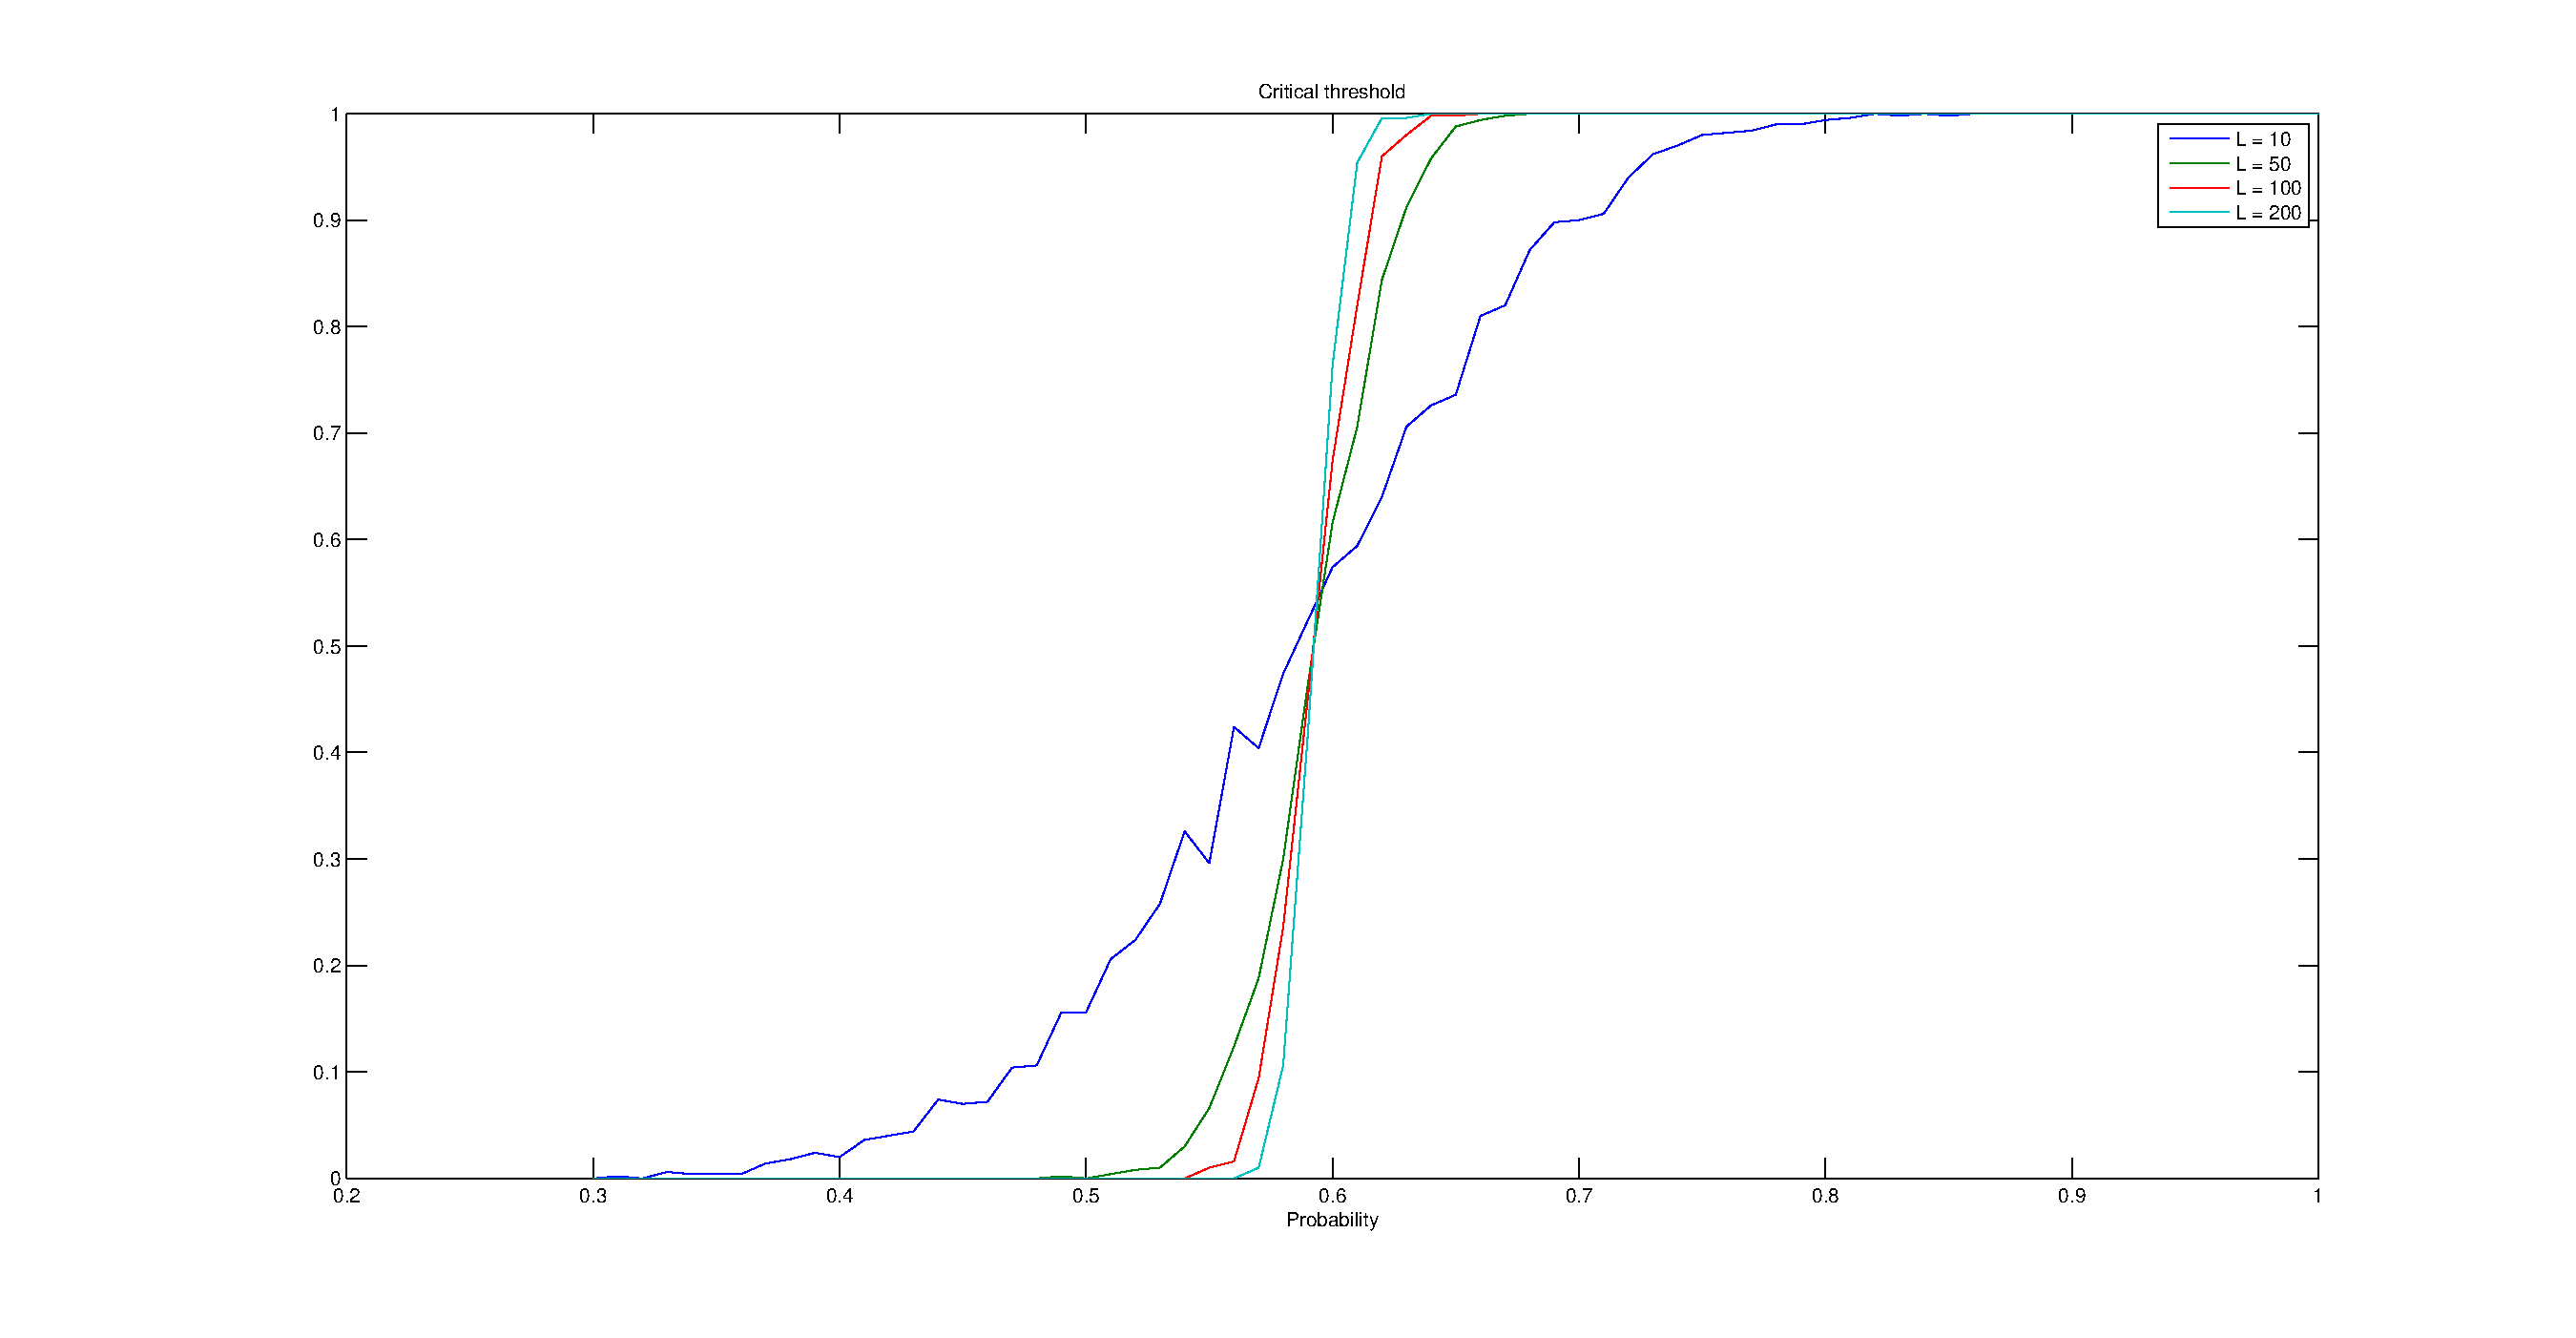
\includegraphics[scale=0.5]{pc.eps}}

Come è possibile notare più il reticolo è grande più è rapida la salita, infatti per reticoli infiniti si avrebbe una funzione a gradino.
\subsection{algoritmo per il calcolo della soglia critica}
L'algoritmo per calcolo della soglia critica, per ogni probabilità \emph{p} da 0.3 a 1 con passo 0.01, per un numero di tentativi, definito dall'utente, crea il reticolo con dimensioni e probabilità \emph{p} differenti e analizza il numero di percolazioni e calcola la media delle percolazioni per ogni probabilità, infine i dati delle medie di percolazioni vengono "plottate" tramite la funzione plot di matlab.\\

\begin{lstlisting}[caption={critical\_threshold.m},label=useless]
function res = critical_threshold(attempts)
  percolation = zeros(1, attempts);
  percolations = [];
  avgPercolations = [];
  AVGpercolation = [];
  AVGpercolation1 = [];
  AVGpercolation2 = [];
  AVGpercolation3 = [];
  x = [];
  xx = [];
  err = [];
    
  for p = 0.3 : 0.01 : 1
    for j = 1 :  attempts
      percolation(j) = cluster_finding(10, p);
    end
    AVGpercolation = [AVGpercolation (mean(percolation))];
    percolation = zeros(1, attempts) ;
    x = [x (p)];
        
    for j = 1 :  attempts
      percolation(j) = cluster_finding(50, p);
    end
    AVGpercolation1 = [AVGpercolation1 (mean(percolation))];
    percolation =zeros(1, attempts) ;
       
    for j = 1 :  attempts
      percolation(j) = cluster_finding(100, p);
    end
    AVGpercolation2 = [AVGpercolation2 (mean(percolation))];
    percolation =zeros(1, attempts) ;
        
    for j = 1 :  attempts
      percolation(j) = cluster_finding(200, p);
    end
    AVGpercolation3 = [AVGpercolation3 (mean(percolation))];
    percolation =zeros(1, attempts) ;
  end
  plot(x,AVGpercolation, 
       x,AVGpercolation1, 
       x,AVGpercolation2, 
       x,AVGpercolation3);
       
  title('Critical threshold');
  xlabel('Probability');
  legend('L = 10', 'L = 50', 'L = 100', 'L = 200');
end
\end{lstlisting}
\section{Reduced average cluster size (RACS)}
Un'altro metodo per trovare la soglia critica è il calcolo del RACS, ovvero la media delle dimensioni dei cluster esclusa del cluster con dimensione massima:\\\\
\[RACS \ = \ \frac{\sum_{s \neq s_{max}}s^2n_{s}}{\sum_{s}sn_{s}} \\ \]\\\\
Analizzando il RACS per diversi valori di L, otteniamo come ci aspettavamo che in prossimità del valore di probabilità  \emph{0.6}\\ la dimensione dei cluster aumenta.

\centerline{\includegraphics[scale=0.5]{racs.eps}}

\subsection{Algoritmo per calcolo del valore RACS}
L'algoritmo per differenti valori di probabilità e differenti dimensioni del reticolo, calcola il valore di RACS, e visualizza i dati tramite un plot.\\
\begin{lstlisting}[caption={calculate\_RACS.m}, label=usless]
function[RACS] = calculate_RACS()
  xx = [];
  totRACS= [];
  avgRACS1 = [];
  avgRACS2 = [];
  avgRACS3 = [];
  avgRACS4 = [];
  for i = 0.1 : 0.04 : 09  %probability
    for j = 1 : 10  %different attempts 
      [found clusters] = cluster_finding(100, i);
      clusters(clusters == max(clusters)) = [];
      RACS = sum(clusters.^2) / sum(clusters);
      totRACS = [totRACS mean(RACS)];
    end
    avgRACS1 = [avgRACS1 mean(totRACS)];
    totRACS = [];
    xx = [xx (i)];
        
    for j = 1 : 5
      [found clusters] = cluster_finding(200, i);
      clusters(clusters == max(clusters)) = [];
      RACS = sum(clusters.^2) / sum(clusters);
      totRACS = [totRACS mean(RACS)];
    end
    avgRACS2 = [avgRACS2 mean(totRACS)];
    totRACS = [];
        
    for j = 1 : 4
      [found clusters] = cluster_finding(400, i);
      clusters(clusters == max(clusters)) = [];
      RACS = sum(clusters.^2) / sum(clusters);
      totRACS = [totRACS mean(RACS)];
    end
    avgRACS3 = [avgRACS3 mean(totRACS)];
    totRACS = [];
        
    for j = 1 : 2
      [found clusters] = cluster_finding(600, i);
      clusters(clusters == max(clusters)) = [];
      RACS = sum(clusters.^2) / sum(clusters);
      totRACS = [totRACS mean(RACS)];
    end
    avgRACS4 = [avgRACS4 mean(totRACS)];
    totRACS = [];
  end
    
  plot(xx, avgRACS1, 
       xx, avgRACS2,
       xx, avgRACS3, 
       xx, avgRACS4);
       
  xlabel('Probability');
  ylabel('Cluster sizes');
  title('Reduced Average Cluster Size');
  legend('L = 100', 
         'L = 200', 
         'L = 400', 'L = 600'); 
  axis([0.2 0.8 0 2500]);
end
\end{lstlisting}
\subsection{Valori di p1, p2, p3}
Indichiamo con p1 la probabilità che un sito del reticolo sia nel cluster massimo, p2 la probabilità che  un sito colorato sia nel cluster massimo e p3 la probabilità che un sito preso tra i cluster sia nel cluster massimo, che sono così definiti:\\\\
\[ p1 = \frac{S_{max}}{L^2};  \ \ \ p2 = \frac{S_{max}}{L^2p};  \ \ \ p3 = \frac{S_{max}}{\sum_{s}Sn_{s}} \]\\\\
Con differenti valori di probabilità e dimensioni dei reticoli, sono stati calcolati i valori di p1, p2 e p3 e come è possibile notare dai grafici, all’aumentare della taglia c’è uno stacco al punto p = 0.6. Si conclude che maggiore è la probabilità di  trovarsi nel cluster massimo maggiore è la  probabilità di vedere il cluster percolante, probabilmente il cluster massimo coincide con quello percolante.

\centerline{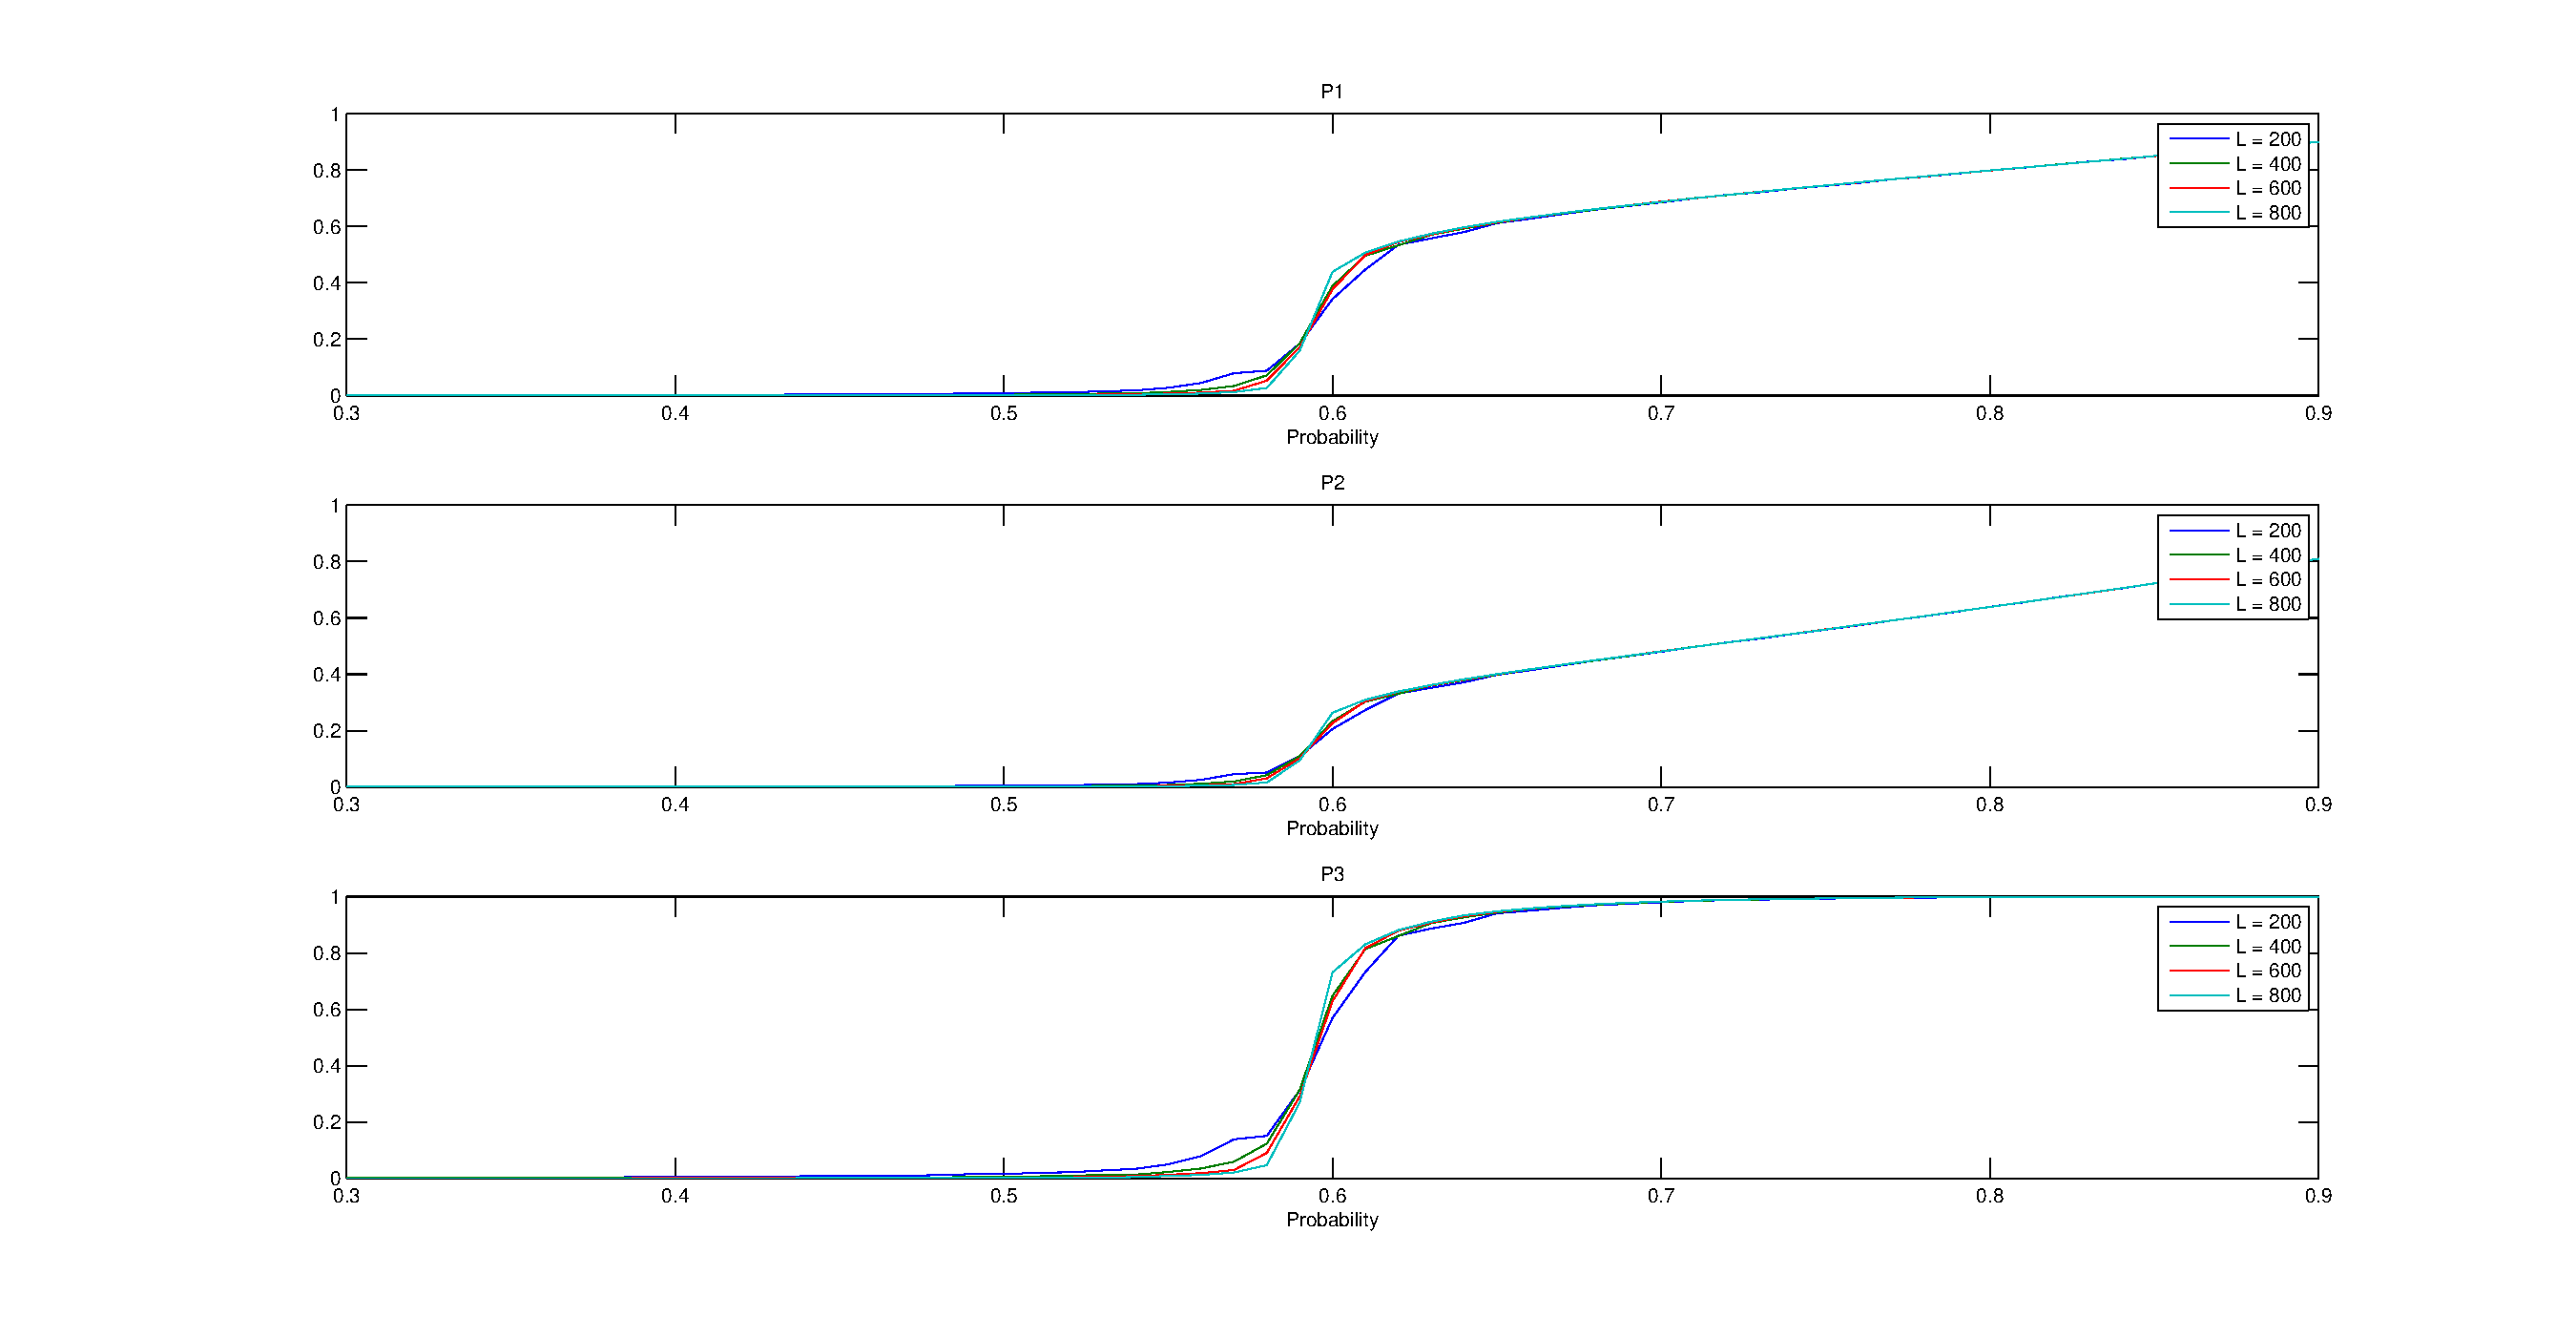
\includegraphics[scale=0.5]{p123.eps}}

\subsection{Algoritmo per il calcolo dei valori di p1, p2 e p3}
Calcolo dei valori di p1, p2 e p3:\\
\begin{lstlisting}[caption={probability\_max\_cluster.m}, label=usless]
function [p1 p2 p3] = probability_max_cluster(N, attempts)
  p1 = zeros(1, attempts);
  p2 = zeros(1, attempts);
  p3 = zeros(1, attempts);
  avgP1 = [];
  avgP2 = [];
  avgP3 = [];
  for p = 0.3 : 0.01 : 1
    for i = 1 : attempts
      [found clusters] =  cluster_finding(N, p);
          
      p1(i) = (max(clusters) / N^2);
      p2(i) = (max(clusters) / (N^2)*p);
      p3(i) = (max(clusters) / sum(clusters));
    end
    avgP1 = [avgP1 mean(p1)];
    avgP2 = [avgP2 mean(p2)];
    avgP3 = [avgP3 mean(p3)];
            
    p1  = zeros(1, attempts);
    p2 = zeros(1, attempts);
    p3 = zeros(1, attempts);
  end
  p1 = avgP1;
  p2 = avgP2;
  p3 = avgP3;
end
\end{lstlisting}
Calcolo per differenti tentativi e dimensioni del reticolo\\
\begin{lstlisting}[caption={percolation.m}, label=usless]
function res = percolation()
  p1 = [];
  p2 = [];
  p3 = [];
  p4 = [];
  p5 = [];
  p6 = [];
  p7 = [];
  p8 = [];
  p9 = [];
  p10 = [];
  p11 = [];
  p12 = [];
  x = 0.3 : 0.01 : 1;
   
  [p1 p2 p3] = probability_max_cluster(200, 10);
  [p4 p5 p6] = probability_max_cluster(400, 10);
  [p7 p8 p9] = probability_max_cluster(600, 10);
  [p10 p11 p12] = probability_max_cluster(800, 10);
    
  subplot(3, 1, 1); 
  plot(x,p1, x,p4, x,p7, x,p10);
  title('P1');
  xlabel('Probability');
  axis([0.3 0.9 0 1]);
  legend('L = 200', 
         'L = 400', 
         'L = 600', 
         'L = 800');
  subplot(3, 1, 2); 
  plot(x,p2, x,p5, x,p8, x,p11);
  title('P2');
  xlabel('Probability');
  axis([0.3 0.9 0 1]);
  legend('L = 200', 
         'L = 400', 
         'L = 600', 
         'L = 800');
  subplot(3, 1, 3); 
  plot(x,p3, x,p6, x,p9, x,p12);
  title('P3');
  xlabel('Probability');
  axis([0.3 0.9 0 1]);
  legend('L = 200', 
         'L = 400', 
         'L = 600', 
         'L = 800');
end
\end{lstlisting}
\section{Calcolo errore e varianza}
In seguito verrà calcolato l’errore relativo a ogni probabilità per la funzione soglia critica:
\begin{lstlisting}[caption={error\_probability.m}, label=usless]
function res = error_probability(N, attempts)
  avgP1 = [];
  avgP2 = [];
  avgP3 = [];
  percolation = [];
  avgPercolation = [];
  err = [];
  x = [];
    
  for p = 0.3 : 0.01 : 1
    for i = 1 : 10
      for j = 1 : attempts / 10
        percolation = [percolation cluster_finding(N, p)];
      end
      avgPercolation = [avgPercolation mean(percolation)];
    end
    err = [err sum(var(avgPercolation))/sqrt(10)];
    avgPercolation = [];
    x = [x p];
  end
  res = mean(err);
  plot(x, err);
  title('Error critical threshold');
  xlabel('Porbability');
end
\end{lstlisting}
\newpage
In seguito possiamo analizzare l'errore per differenti probabilità, 100 tentativi e dimensione del reticolo = 200:

\centerline{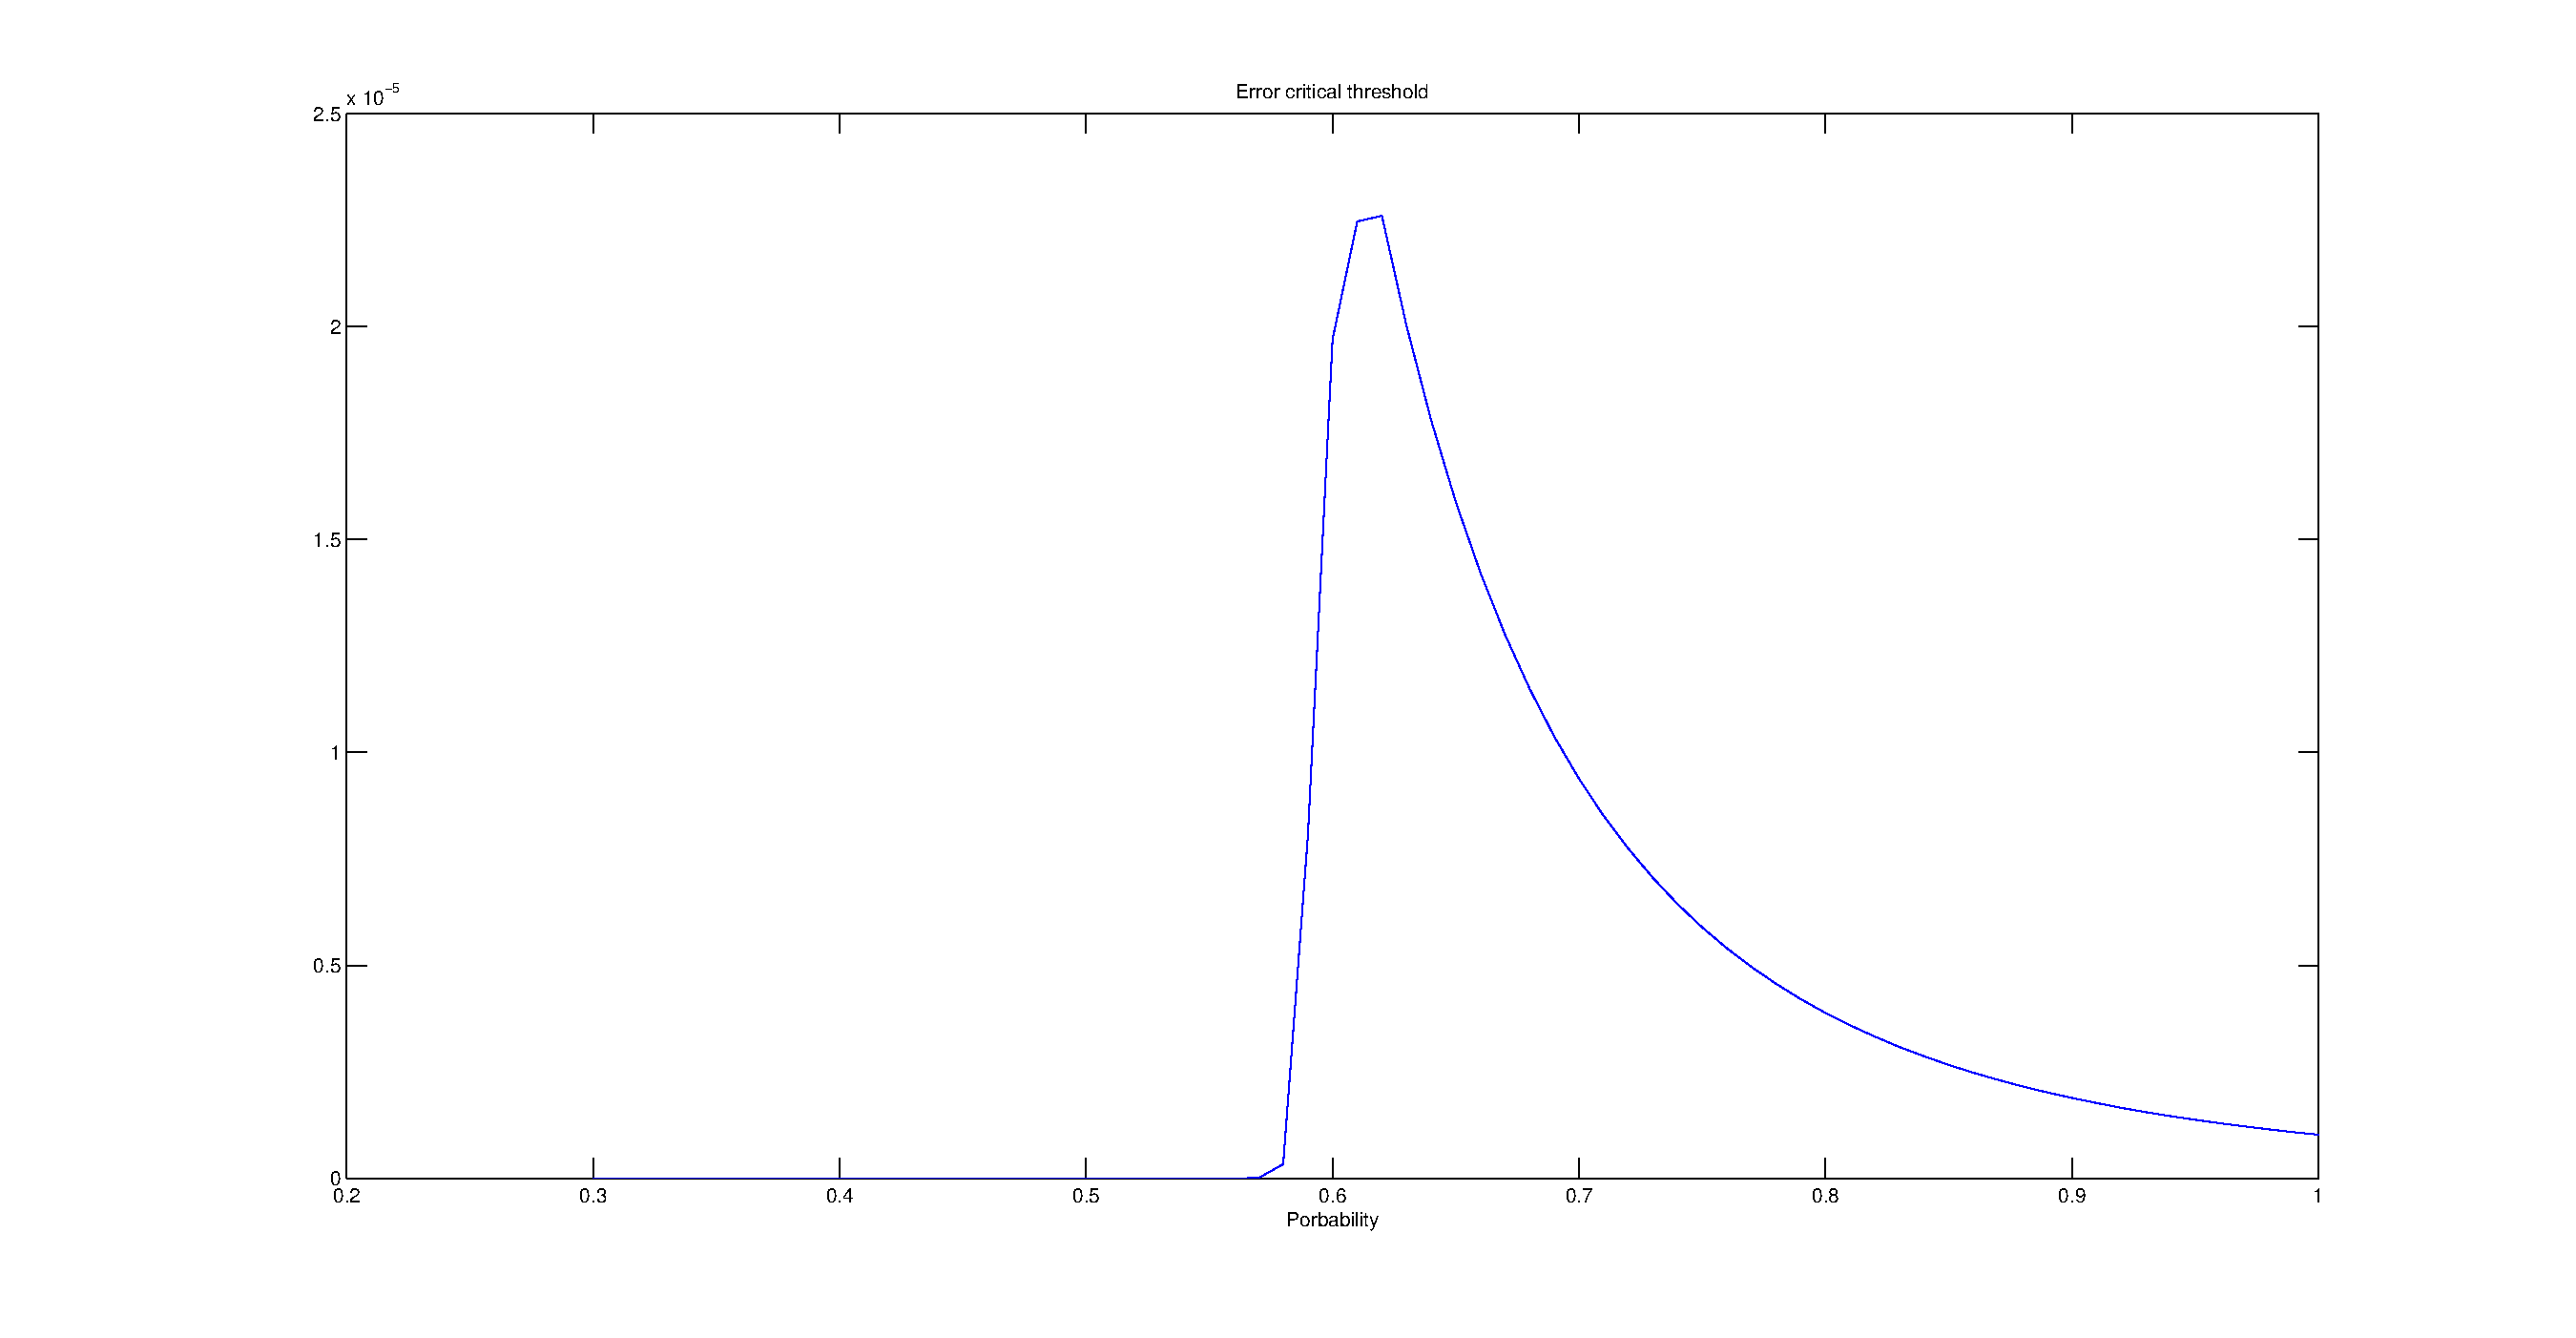
\includegraphics[scale=0.5]{error.eps}}

\section{Algoritmo HK}
L'algoritmo di Hoshen-Kopelman visita l'intero reticolo, sito per sito partendo dallo spigolo in alto a sinistra per arrivaro a quello in basso a destra. Quando incontra un sito occupato che non è connesso ad altri siti occupati in alto o a sinistra inizia un nuovo cluster e viene assegnato al sito una nuova label. Se invece c'è un sito occupato vicino in alto o a sinistra, il sito che si sta analizzando prende la label di un sito vicino occupato, analogamente per i suoi primi vicini sono entrambi occupati e con la stessa label. \\
\begin{center}
\includegraphics[scale=0.6]{cl1.png}
\end{center}
Durante l'analisi del reticolo può capitare di incontrare "collisioni" di label
\begin{center}
\includegraphics[scale=0.6]{cl2.png}
\end{center}
in questo caso si sceglie la label con valore minore, anche se appartiene allo stesso cluster, modificare le label dei siti vicini comporterebbe troppo tempo. Soltanto in seguito verra fatto il "relabeling" per assegnare ai cluster il valore label corretto.\\
Di seguito l'implementazione dell'algoritmo di HK:\\
\begin{lstlisting}[caption={HK\_algorithm.m}, label=usless]
function [found sizes clusters] = HK_algorithm(N, p) 
  randMatrix = rand(N);
  Matrix = zeros(N);
  Matrix(randMatrix < p) = 1;
     
  labels = [];
  totLabels = 0;
  found = 0;
  N = size(Matrix);
    
  for i = 1 : N
    for j = 1 : N
      if(Matrix(i, j) == 1)
        up = 0;
        left = 0;    
        if(i > 1)
          up = Matrix(i-1, j);
        end     
        if(j > 1)
          left = Matrix(i, j-1);
        end
                
        switch((up > 0) + (left > 0))
          %new cluster
          case 0
            totLabels = totLabels + 1;
            labels(totLabels) = totLabels;
            Matrix(i, j) = totLabels;
                  
          %same cluster
          case 1
            Matrix(i, j) = up + left;
                       
          %different cluster
          case 2
            while labels(up) < up
              up = labels(up);
            end
                        
            while labels(left) < left
              left = labels(left);
            end
            Matrix(i, j) = min([up left]);
            labels(max([up left])) = min([up left]);
        end % switch
      end % if 
    end % for
  end % for
    
  %renaming labels array
  j = 1;
  for i = 1 : totLabels
    if(labels(i) == i)
      labels(i) = j;
        j = j +1;
      else
        labels(i) = labels(labels(i));
    end
  end
    
  %apply the labels array to the matrix
  for i = 1 : N
    for j = 1 : N
      if(Matrix(i, j) ~= 0)
        Matrix(i, j) = labels(Matrix(i, j));
      end
    end
  end
    
  sizes = [];
  for i = 1 : max(labels)
    sizes = [sizes length(find(Matrix == i))];
  end
    
  count = 0;
  for i = 1 : max(labels)
    for j = 1 : N
      if(~isempty(find(Matrix(:, j) == i, 1)))
        count = count + 1;
      end
      if(count == N)
        found = 1;
        clusters = Matrix;
        return;
      end
    end
    count = 0;
  end      
end
\end{lstlisting}
\end{document}
